\subsection{Window-System}

\subsubsection{Fenster}
Ein Spiel \textit{"`passiert"'} in unserem heutigen Zeitalter wie jedes andere GUI in einem \textit{Fenster}. Um ein solches zu erstellen wurde in der FM3D-Engine die Klassen \textit{Window} und \textit{Win32Window} implementiert.
Window ist die Basisklasse, von welcher alle Fenstertypen erben sollen.
Die Klasse besitzt die Attribute \textit{width} und \textit{heigth} vom Typ Integer, welche die Breite und Höhe eines Fensters darstellen.
Es existieren ein Konstruktor und verschiedene Methoden, die die Interaktion mit einem Fenster ermöglichen. Alles erwähnte ist \textit{protected}.
\textit{Start} startet unter Angabe der Parameter, welche die Breite, Höhe, den Fenster Titel, und die Sichtbarkeit des Fensters angeben, das bereits erstellte Fenster.
Die Methode HasMessage gibt an ob das Fenster eine Message hat und
Shouldclose gibt zurück ob das Fenster geschlossen werden soll.
Die Methode \textit{Close()} schließt ein Fenster. Mit der Methode Create() erstellt man ein neues Fenster mit den Übergabeparametern der Plattform auf welchem das Spiel bzw. die GUI laufen soll und einem Objekt der Klasse HINSTANCE, welches ein Handle für Windows-Anwendungen ist. Die Methode \textit{StartConsole()} startet eine Konsole für eventuelle Fehlerdiagnosen oder ähnliches. Mit der Methode \textit{SetConsolePosition} kann man nun mit Übergabeparametern X und Y vom Typ Integer, die Koordinaten auf dem Bildschirm beschreiben, die Position der Konsole auf dem Bildschirm setzen.
Jedes \textit{Window}-Objekt besitzt ein Objekt der Klasse Input, doch dazu später mehr. Die Basistklasse \textit{Window} hat den Vorteil, dass man verschiedene Fensterklassen für verschiedene Betriebssysteme implementieren könnte. In der aktuellen Version der Engine existiert nur eine Fensterklasse für Windows32 die von \textit{Window} erbt. Dies ist die Klasse  \textit{Win32Window}. Die Klasse Windows besitzt zudem noch einige \textit{Get-} und \textit{Set-}Methoden unteranderem für die Größe und Position des Fensters auf dem Bildschirm.

Wie schon erwähnt erbt die Klasse \textit{Windows32Window} von der Klasse \textit{Window} und die Klasse \textit{Window} steht zu \textit{Win32Window} in einer \textit{friend} Beziehung.
\textit{Win32Window} besitzt die Attribute msg vom Typ \textit{MSG}, \textit{hWnd} vom Typ \textit{HWND}, \textit{hInstance} vom Typ \textit{HINSTANCE} und einen String der den Namen des Fensters beschreibt.
HWND ist ein Windowshandle für Fenster und \textit{MSG} ein Windows-Datentyp für Informationen über die Nachrichten eines Threads. 
Die Klasse besitzt zudem einen Konstruktor, dem man ein Objekt der Klasse \textit{HINSTANCE} übergibt, vier \textit{Public} Methoden und eine \textit{Private} Methode. Die Methode Start startet das Fenster und benötigt als Übergabeparameter die Höhe, die Breite, den Titel des Fensters und einen boolschen Wert, der angibt ob das Fenster angezeigt werden soll, oder nicht.
Auch hier gibt die Methode HasMessage an ob das Fenster eine Message hat und
Shouldclose gibt zurück ob das Fenster geschlossen werden soll. Nur sind diese Methoden auf Windows32 zugeschnitten und verwenden unteranderem auch die Methoden aus der Klasse Window.
\textit{Close} schließt das Fenster. (für weitere Informationen Siehe \cref{Windowsystem})

\begin{figure}
	\begin{center}
		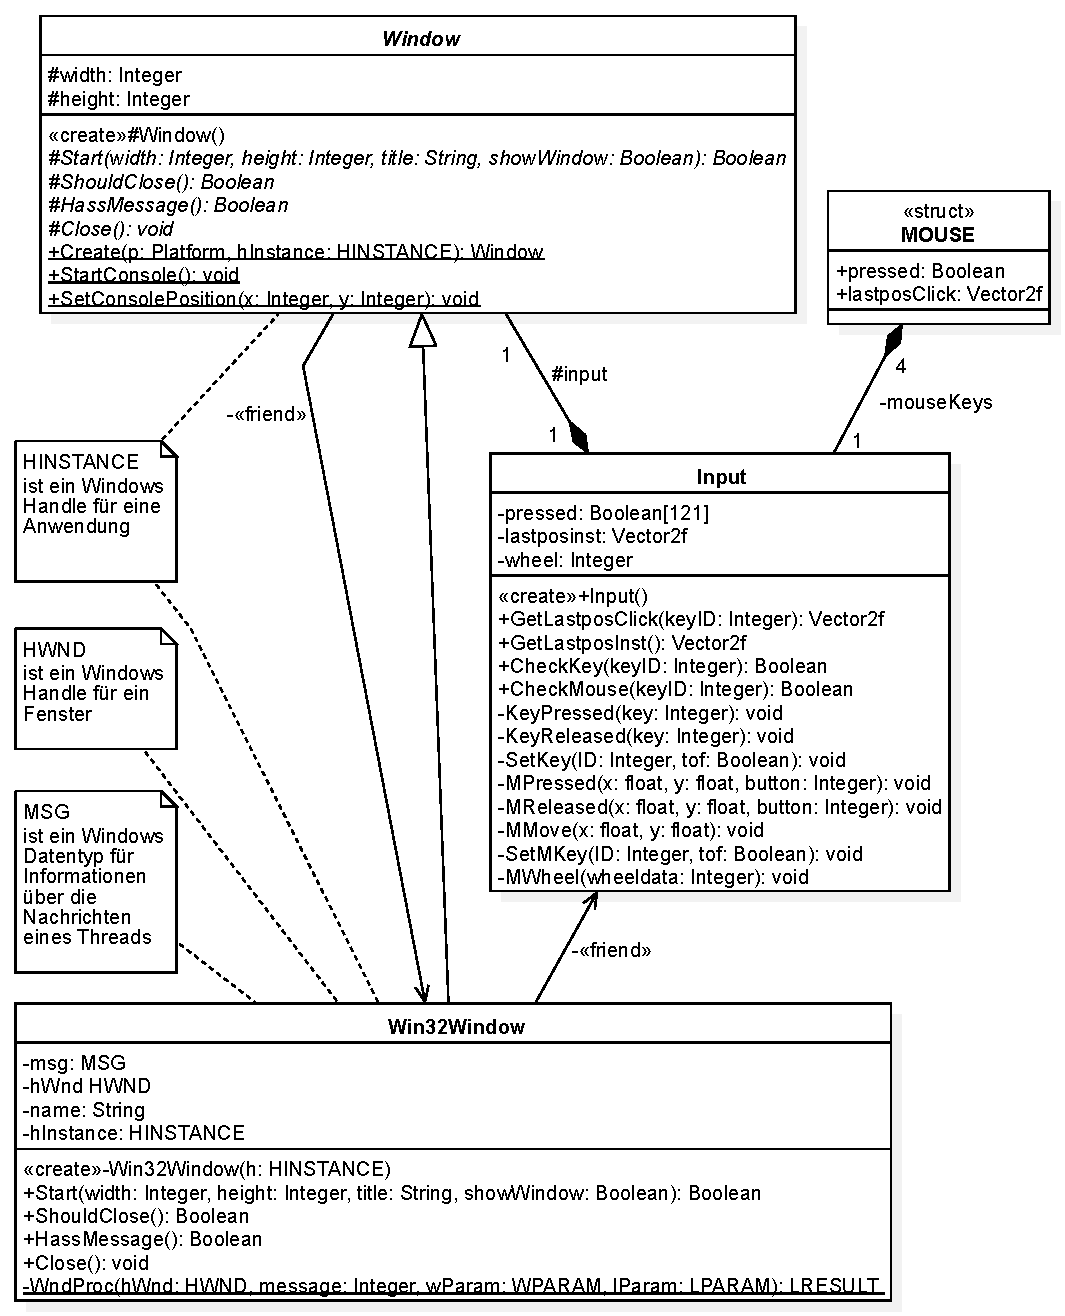
\includegraphics[width=\textwidth]{03unserprogramm/Engine/WindowSystem.pdf}
		Es wurde auf die Angabe von Get- und Set-Methoden sowie Events verzichtet.
		\caption{Window-System}\label{Windowsystem}
	\end{center}
\end{figure}

\subsubsection{Input-Klasse}

Natürlich benötigt ein Spiel bzw. auch die meisten Grafischen Nutzer-Oberflächen auch ein sicheres Eingabe-System, welches sowohl die Position der Maus ermittelt, aber auch die Abfrage jeder einzelnen Taste auf der Tastatur regelt. 
Dafür wurde in der FM3D-Engine eine eigene Klasse implementiert, welche für dies zuständig ist.
Um den Nutzer der FM3D-Engine davor zu bewahren nicht jeden einzelnen ASCII-Code jeder Taste auf der Tastatur nachzuschlagen, sind alle Tasten in Form von Makros definiert. 
In dem Namespace FM3D befindet sich die Klasse \textit{Input} und jedes Objekt eines Fensters bzw. der Klasse \textit{Window} besitzt ein Objekt dieser Klasse. Die Klasse Input beinhaltet außerdem die Enumeration \textit{KEYCLICK}, welches den aktuellen Stand der Maustasten beschreibt. Diese können entweder gedrückt, nicht gedrückt oder losgelassen werden und sind in dieser Enumeration definiert.
Eine Struktur \textit{MOUSE} enthält die Enumeration \textit{KEYCLICK} und einen zweidimensionalen Vektor des Typen \textit{Float}, welcher die zweidimensionale Position im Fenster in OpenGL Koordinaten angibt, an welcher eine Taste der Maus gedrückt wurde.
Diese Struktur wird in der Klasse Input als ein vier-Felder Array verwendet, welches jede Taste einer durchschnittlichen Maus beschreibt. Diese sind die linke, die rechte und die mittlere Maustaste. Das letzte Feld ist für ein zusätzliches Feld einer beliebigen Taste der Maus reserviert, da es immer unterschiedliche Maustypen gibt.
Zudem besitzt die Klasse \textit{Input} einen Vektor \textit{lastposinst}, welcher ununterbrochen die Position der Maus ermittelt. Dies ist in den Spielen erforderlich in denen die Maus ununterbrochen die Kamera steuert.

Für die Tastenabfrage wurde zunächst ein Integer Wert verwendet, in welchen der aktuell gedrückte ASCII-Code gespeichert wurde. Dies hat aber den Nachteil, dass nur eine Taste gedrückt sein bzw. abgefragt werden kann. Möchte man nun zum Beispiel einen Spiele-Charakter schräg durch einen Raum durch gedrückte Links- \textbf{und} Rechts-Taste bewegen, so wäre das mit dieser Möglichkeit nicht möglich. Deswegen beschreibt nun ein 121-Felder Array aus booleschen Werten die komplette Tastatur. Jede Feldnummer ist äquivalent zu dem zugeordneten ASCII-Code der Taste. Die Felder [1] bis [4] beschreiben die Maustasten. Einige Felder des Arrays sind nicht von einem ASCII Code auf der Tastatur \textit{belegt} und sind somit "`\textit{frei}"'. Dies hat den Vorteil, dass später simpel weitere Eingabegeräte in das Inputsystem eingebunden werden können.
Die Klasse besitzt Methoden, welche in der Klasse Win32Window.h (Siehe Doxygen Dokumentation), die ein GUI-Fenster abbildet, die die verschiedenen Werte der Arrays und des Vektors setzen.
Zudem besitzt die Klasse Methoden, die diese Werte zurück geben. (Für die Verwendung dieser Klasse siehe \cref{inputsystemver})